\documentclass[12pt,a4paper]{article}

% --- Essential Packages ---
\usepackage[utf8]{inputenc}
\usepackage{geometry}
\geometry{a4paper, margin=1in}
\usepackage{amsmath}
\usepackage{graphicx}
\usepackage{hyperref}
\usepackage{subcaption}
\usepackage{float}

% --- Hyperlink Colors ---
\hypersetup{
    colorlinks=true,
    linkcolor=blue,
    urlcolor=cyan
}

% --- Title Page Info ---
\title{
     \vspace*{1cm}
    
\includegraphics[width=6cm]{../report/assets/logo.png} \\
    \vspace*{1cm}
    \large Brno University of Technology \\
    \large Faculty of Information Technology \\
    \vspace{2cm}

    \textbf{Image Processing Filter Effects} \\
    \vspace*{1cm}
    \large Project Report\\
    \vspace{1cm}
    \large{ZPOe 25/26} \\
    \vspace{1cm}
    \vspace*{1cm}
    \large Adar Otieno - xotiena00\\
    \large Deniz Aksoy - xaksoyd00\\
    \large Eyobed Awel Nuri - xnuriey00\\
    \vfill
    \date{\today}
}

\begin{document}

\maketitle
\newpage

\tableofcontents
\newpage

% --- Main Content ---

\section{Introduction}
In the field of computer vision and image processing, filters are essential tools used to manipulate and analyze images. They operate by modifying the pixels of an image based on mathematical functions, allowing for enhancements, artistic effects, or noise reduction. 

This project explores the implementation of custom image filters using C++ and the OpenCV library. Rather than relying entirely on pre-built, high-level OpenCV functions, the focus of this work is on the manual, pixel-by-pixel implementation of various effects to understand the underlying mathematics and algorithms. The application serves as an interactive GUI that allows users to seamlessly apply and switch between 12 unique filters developed by the team.

\subsection{Project Architecture}
The core application is built as a single interactive window utilizing OpenCV's HighGUI module. The architecture emphasizes modularity, ensuring that each contributor can develop their effects independently. 

The application utilizes a \texttt{Filter} structure to register the effects:
\begin{verbatim}
struct Filter {
  string author;
  string name;
  string description;
  Mat (*apply)(const Mat &);
};
\end{verbatim}

This structure enables the main application to dynamically load the filters, populate the trackbar controls, and render an informative metadata panel detailing the active effect and its creator.

\section{Implementation Details}
The project incorporates a total of 12 distinct filters, divided equally among the three contributors: Eyobed, Adar, and Denis.

\subsection{Eyobed's Filters}
\begin{itemize}
    \item \textbf{Histogram Equalization:} Enhances image contrast by redistributing the brightness values across the full 0-255 range. To prevent unwanted color shifting, the algorithm operates in the YCrCb color space, applying the equalization solely to the luminance (Y) channel before converting back to BGR.
    \item \textbf{Lens Distortion:} Applies a manual barrel distortion effect, simulating the physical curvature of a camera lens. The pixels are mapped using a radial geometric transform.
    \item \textbf{Zoom Blur:} A radial blur effect that streaks pixels from the edges of the image towards the center. This is achieved using a manually implemented directional box blur kernel.
    \item \textbf{Posterize:} Reduces the continuous color palette into a limited number of discrete values. This manual color quantization gives the image a distinct comic-book or retro-art aesthetic.
\end{itemize}

\subsection{Adar's Filters}
Adar's contributions focus on manual pixel manipulation using native loops, avoiding optimized OpenCV functions for educational purposes.
\begin{itemize}
    \item \textbf{Relief Emboss:} Creates a 3D gray relief texture by subtracting the bottom-right neighboring pixel from the top-left neighbor and adding an offset of 128 to center the result.
    \item \textbf{Dodge:} Implements the classic Color Dodge blend formula: \texttt{(pixel * 255) / max(1, 255 - pixel)}. This blows out the highlights and drastically increases contrast.
    \item \textbf{Swirl:} Warps the image into a vortex by converting Cartesian coordinates to Polar coordinates, applying a nonlinear rotational offset based on the radius, and converting back to sample the pixel.
    \item \textbf{Bloom:} Extracts bright pixels (intensity $>$ 180) and applies a brute-force nested 7x7 loop to blur them. The resulting glow is then added directly back to the original image.
\end{itemize}

\subsection{Deniz's Filters}

Similar to Adar, Deniz's filters prioritize foundational image processing algorithms implemented through direct pixel-by-pixel matrix iteration. The objective of these filters is not only to produce visually interesting effects but also to demonstrate the mathematical principles behind image segmentation, stochastic distortion, procedural rendering, and color-space manipulation.

\subsubsection{Original Input Images}

The following images were selected as the common input dataset for evaluating the visual behavior and robustness of the implemented filters.

\begin{figure}[H]
    \centering

    \begin{subfigure}{0.23\textwidth}
        \centering
        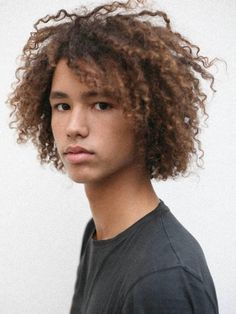
\includegraphics[width=\linewidth]{assets/cross_original_1.jpg}
        \caption{Input 1}
    \end{subfigure}
    \hfill
    \begin{subfigure}{0.23\textwidth}
        \centering
        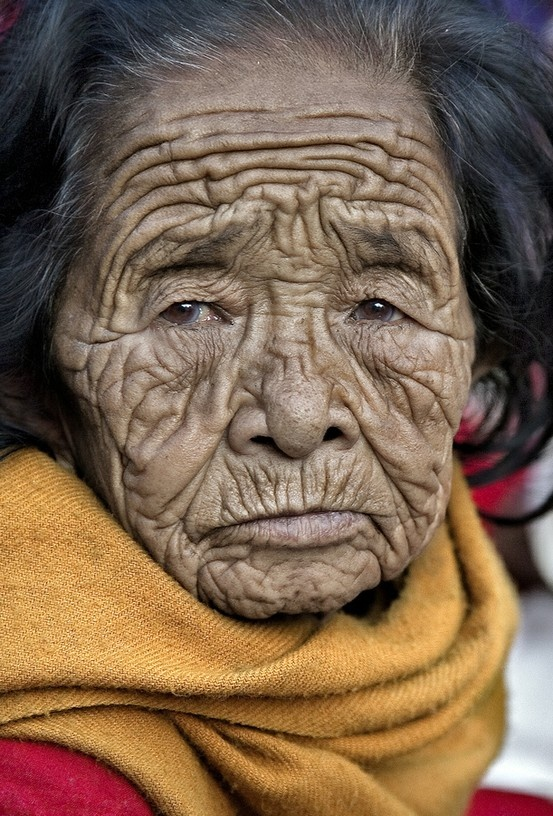
\includegraphics[width=\linewidth]{assets/cross_original_2.jpg}
        \caption{Input 2}
    \end{subfigure}
    \hfill
    \begin{subfigure}{0.23\textwidth}
        \centering
        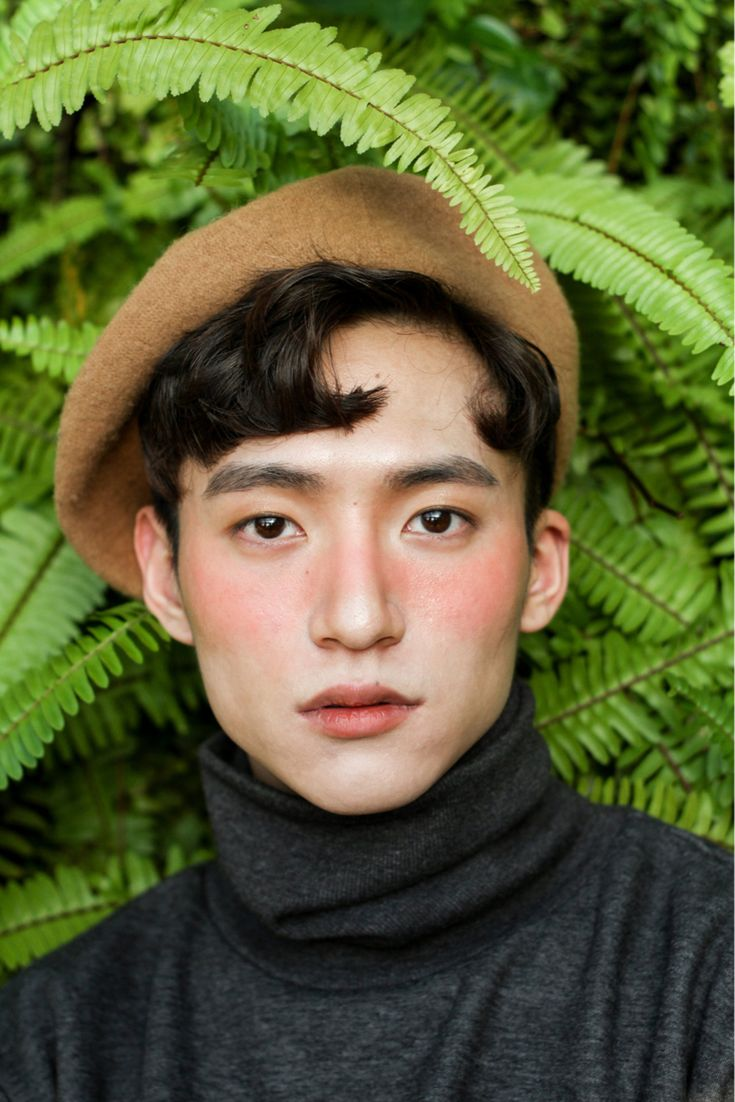
\includegraphics[width=\linewidth]{assets/cross_original_3.jpg}
        \caption{Input 3}
    \end{subfigure}
    \hfill
    \begin{subfigure}{0.23\textwidth}
        \centering
        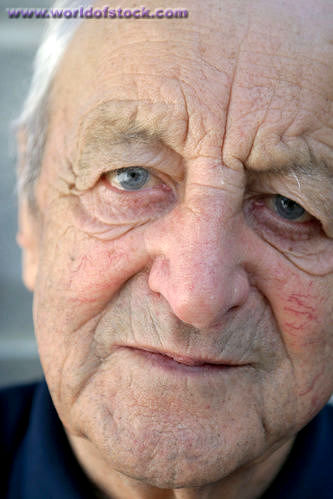
\includegraphics[width=\linewidth]{assets/cross_original_4.jpg}
        \caption{Input 4}
    \end{subfigure}

    \caption{Original input images used for evaluating Denis's image processing filters.}
    \label{fig:original_inputs}
\end{figure}

\subsubsection{Threshold Filter}

The Threshold filter is a classical image segmentation and binarization technique used to separate foreground information from the background. The implementation manually iterates through every pixel and computes its luminosity value using the weighted grayscale conversion formula:

\[
L = 0.299R + 0.587G + 0.114B
\]

This weighted grayscale formula reflects the sensitivity of the human visual system, which perceives green wavelengths more strongly than blue wavelengths. After computing the luminosity, a binary threshold operation is applied:

\[
\text{Output} =
\begin{cases}
255, & \text{if } L > T \\
0, & \text{otherwise}
\end{cases}
\]

where \(T\) denotes the threshold value.

Thresholding belongs to the category of binary image processing and is widely used in OCR systems, edge detection, document analysis, license plate recognition, and preprocessing pipelines for machine learning applications.

The computational complexity of the algorithm is:

\[
O(W \times H)
\]

where \(W\) and \(H\) represent the width and height of the image respectively.

\begin{figure}[H]
    \centering

    \begin{subfigure}{0.23\textwidth}
    \centering
    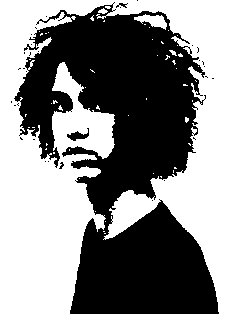
\includegraphics[width=\linewidth]{assets/threshold_1.png}
    \caption{Result 1}
\end{subfigure}
\hfill
\begin{subfigure}{0.23\textwidth}
    \centering
    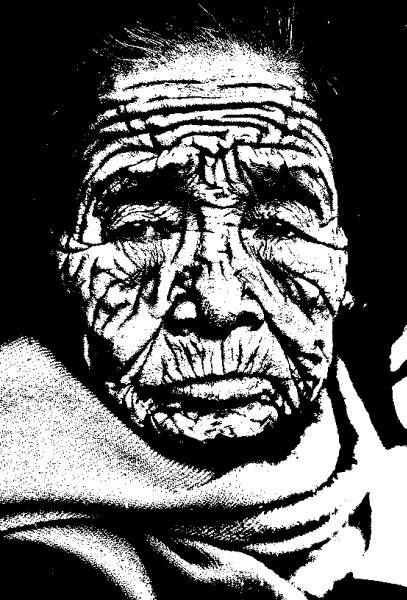
\includegraphics[width=\linewidth]{assets/threshold_2.png}
    \caption{Result 2}
\end{subfigure}
\hfill
\begin{subfigure}{0.23\textwidth}
    \centering
    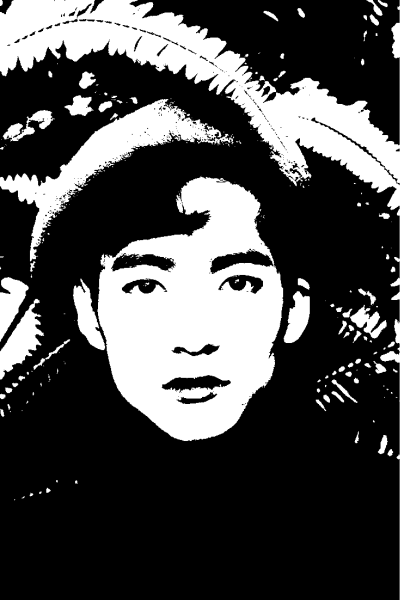
\includegraphics[width=\linewidth]{assets/threshold_3.png}
    \caption{Result 3}
\end{subfigure}
\hfill
\begin{subfigure}{0.23\textwidth}
    \centering
    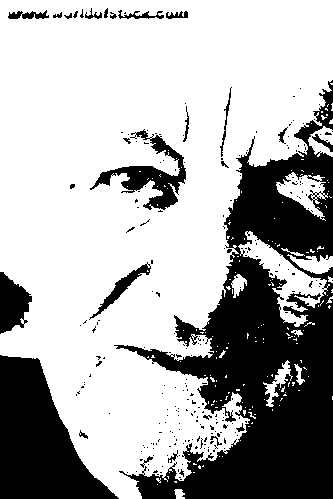
\includegraphics[width=\linewidth]{assets/threshold_4.png}
    \caption{Result 4}
\end{subfigure}

    \caption{Results after applying the Threshold filter to the original images shown in Figure~\ref{fig:original_inputs}.}
    \label{fig:threshold_results}
\end{figure}

\subsubsection{Diffuse Filter}

The Diffuse filter creates a frosted-glass distortion effect by replacing each pixel with a randomly selected neighboring pixel located within a predefined radius. Unlike traditional blur filters that average neighboring pixels, the diffuse filter uses stochastic sampling to introduce randomized local distortion.

For a given pixel coordinate \((x,y)\), a neighboring pixel is selected according to:

\[
(x', y') = (x + r_x,\ y + r_y)
\]

where \(r_x\) and \(r_y\) are random offsets constrained within the selected radius.

This process creates an organic scattering effect that resembles viewing an object through textured or frosted glass. The filter belongs to the category of artistic image stylization and non-linear image distortion.

The algorithm is computationally linear:

\[
O(W \times H)
\]

although random memory access patterns may slightly reduce cache efficiency compared to standard convolution-based methods.

\begin{figure}[H]
    \centering

    \begin{subfigure}{0.23\textwidth}
    \centering
    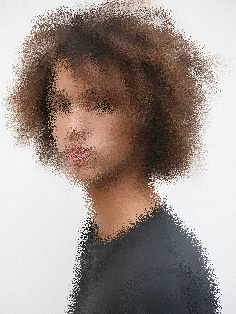
\includegraphics[width=\linewidth]{assets/diffuse_1.png}
    \caption{Result 1}
\end{subfigure}
\hfill
\begin{subfigure}{0.23\textwidth}
    \centering
    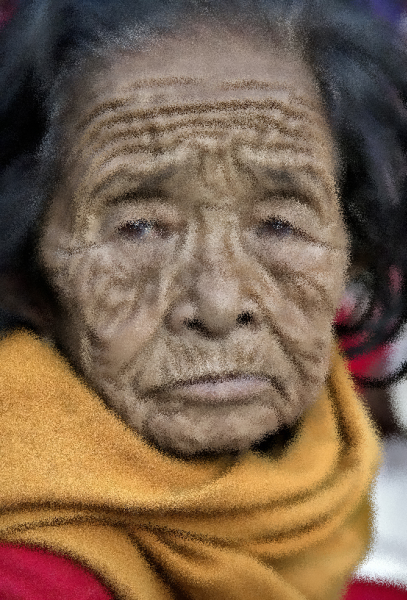
\includegraphics[width=\linewidth]{assets/diffuse_2.png}
    \caption{Result 2}
\end{subfigure}
\hfill
\begin{subfigure}{0.23\textwidth}
    \centering
    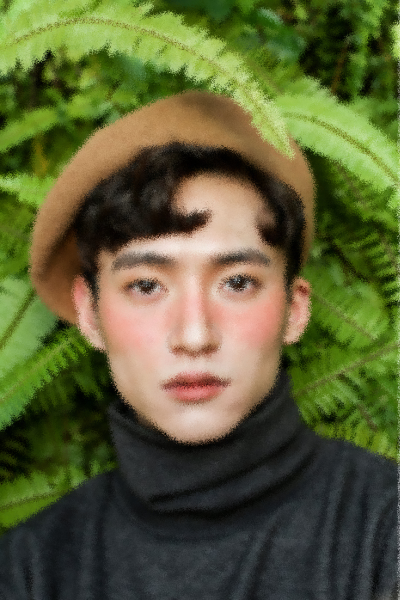
\includegraphics[width=\linewidth]{assets/diffuse_3.png}
    \caption{Result 3}
\end{subfigure}
\hfill
\begin{subfigure}{0.23\textwidth}
    \centering
    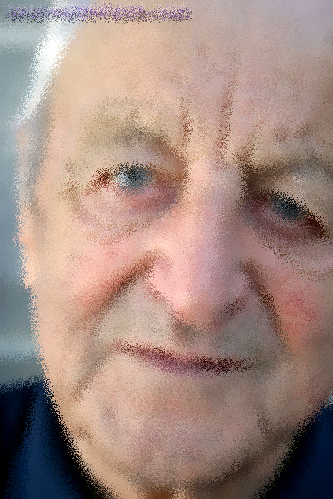
\includegraphics[width=\linewidth]{assets/diffuse_4.png}
    \caption{Result 4}
\end{subfigure}

    \caption{Results after applying the Diffuse filter to the original images shown in Figure~\ref{fig:original_inputs}.}
    \label{fig:diffuse_results}
\end{figure}

\subsubsection{Crosshatch Filter}

The Crosshatch filter is a non-photorealistic rendering (NPR) technique designed to imitate traditional pen-and-ink sketching methods. Instead of relying on convolution kernels, the filter procedurally generates diagonal line structures using modulo arithmetic on pixel coordinates.

The basic pattern generation can be represented as:

\[
(x + y) \bmod n = 0
\]

where \(n\) controls the spacing between hatch lines.

Additional line layers are introduced depending on the darkness of the underlying pixel. Darker image regions receive denser hatch structures, while brighter regions contain fewer strokes. This behavior simulates classical artistic shading techniques used in traditional crosshatching.

The filter is computationally lightweight and maintains linear complexity:

\[
O(W \times H)
\]

Crosshatching is frequently used in sketch simulation, comic-book rendering, procedural graphics, and artistic visualization systems.

\begin{figure}[H]
    \centering

    \begin{subfigure}{0.23\textwidth}
        \centering
        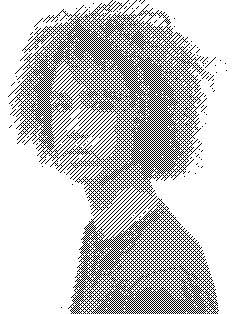
\includegraphics[width=\linewidth]{assets/cross_filtered_1.png}
        \caption{Result 1}
    \end{subfigure}
    \hfill
    \begin{subfigure}{0.23\textwidth}
        \centering
        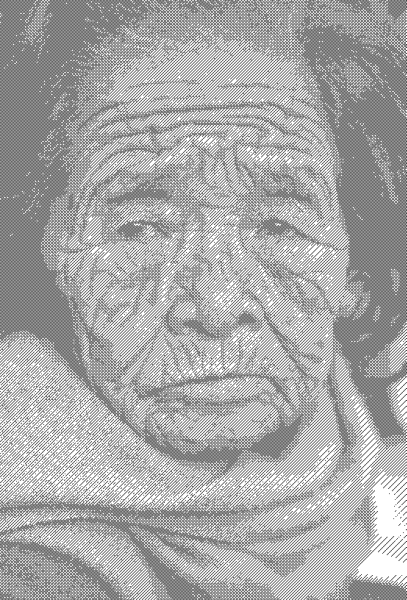
\includegraphics[width=\linewidth]{assets/cross_filtered_2.png}
        \caption{Result 2}
    \end{subfigure}
    \hfill
    \begin{subfigure}{0.23\textwidth}
        \centering
        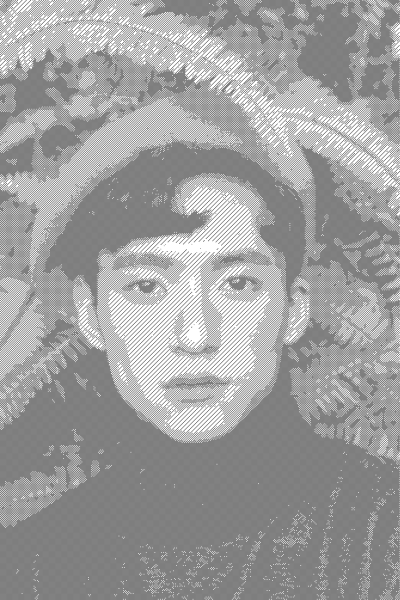
\includegraphics[width=\linewidth]{assets/cross_filtered_3.png}
        \caption{Result 3}
    \end{subfigure}
    \hfill
    \begin{subfigure}{0.23\textwidth}
        \centering
        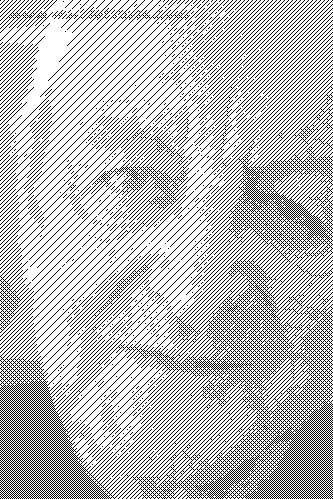
\includegraphics[width=\linewidth]{assets/cross_filtered_4.png}
        \caption{Result 4}
    \end{subfigure}

    \caption{Results after applying the Crosshatch filter to the original images shown in Figure~\ref{fig:original_inputs}.}
    \label{fig:crosshatch_results}
\end{figure}

\subsubsection{Hue Rotate Filter}

The Hue Rotate filter modifies image colors by rotating the Hue channel in the HSV color space. The image is first converted from BGR to HSV using OpenCV before manually modifying the Hue channel.

The hue transformation is computed as:

\[
H' = (H + \Delta H) \bmod 180
\]

where \(\Delta H = 60\) degrees in the implemented effect.

Modulo arithmetic is required because hue values form a circular color wheel. Once the hue exceeds the maximum range, it wraps around to the beginning of the spectrum.

Hue rotation is widely used in artistic color grading, game graphics, data augmentation, augmented reality filters, and image stylization pipelines.

The computational complexity remains:

\[
O(W \times H)
\]

since each pixel is processed independently.

\begin{figure}[H]
    \centering

    \begin{subfigure}{0.23\textwidth}
    \centering
    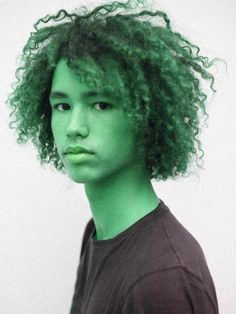
\includegraphics[width=\linewidth]{assets/hue_1.png}
    \caption{Result 1}
\end{subfigure}
\hfill
\begin{subfigure}{0.23\textwidth}
    \centering
    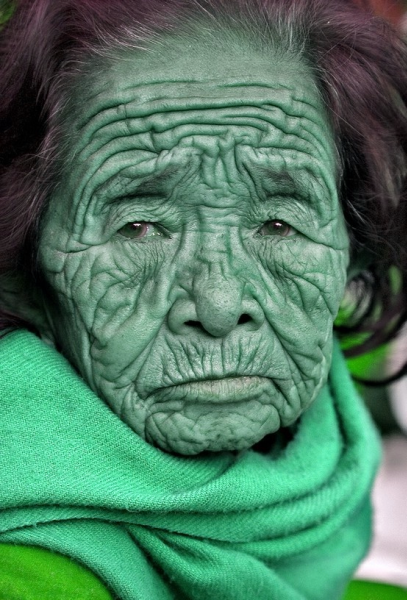
\includegraphics[width=\linewidth]{assets/hue_2.png}
    \caption{Result 2}
\end{subfigure}
\hfill
\begin{subfigure}{0.23\textwidth}
    \centering
    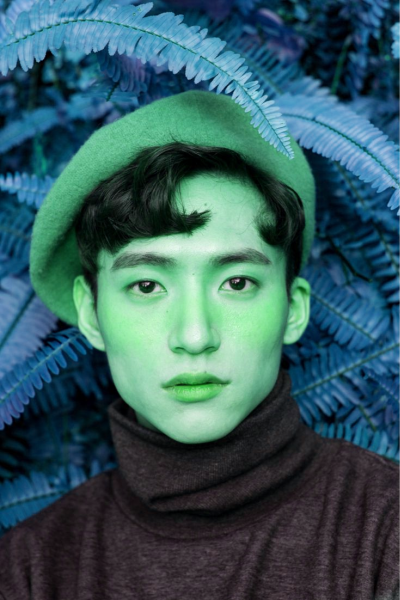
\includegraphics[width=\linewidth]{assets/hue_3.png}
    \caption{Result 3}
\end{subfigure}
\hfill
\begin{subfigure}{0.23\textwidth}
    \centering
    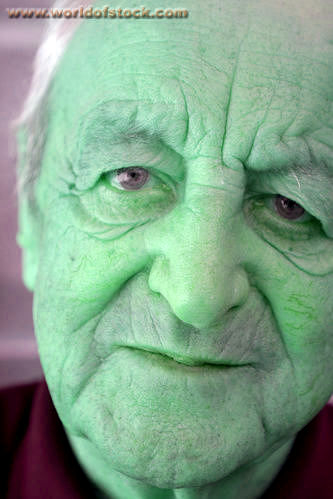
\includegraphics[width=\linewidth]{assets/hue_4.png}
    \caption{Result 4}
\end{subfigure}

    \caption{Results after applying the Hue Rotate filter to the original images shown in Figure~\ref{fig:original_inputs}.}
    \label{fig:hue_results}
\end{figure}
\subsubsection{Evaluation and Discussion}

The implemented filters successfully demonstrate several fundamental concepts in image processing, including binary segmentation, stochastic pixel manipulation, procedural non-photorealistic rendering, and color-space transformation. The Threshold filter proved highly effective for simplifying image structures and emphasizing high-contrast regions, making it particularly suitable for preprocessing tasks such as OCR and edge extraction. The Diffuse filter generated visually organic distortions that simulated frosted-glass effects through randomized neighborhood sampling, although fine image details were partially degraded due to stochastic pixel replacement. The Crosshatch filter effectively transformed photographic content into stylized sketch-like renderings using lightweight mathematical coordinate patterns, demonstrating how procedural line generation can emulate traditional artistic shading techniques. Finally, the Hue Rotate filter showed that manipulating the HSV color space provides an efficient method for altering image appearance while preserving geometric structure and brightness information. Overall, the results confirm that relatively simple pixel-level algorithms can produce both technically meaningful and visually compelling transformations while maintaining computational efficiency with linear time complexity.

\section{Graphical User Interface}
The application provides an intuitive way to visualize the image processing results. It is composed of three primary windows:

\begin{enumerate}
    \item \textbf{Controls:} Houses two OpenCV trackbars. The first trackbar cycles through all available images in the \texttt{data/} directory. The second trackbar cycles through the 12 registered filters.
    \item \textbf{Original / Filtered Views:} Displays the before-and-after results. To ensure a consistent viewing experience, a \texttt{resizeForDisplay()} function scales both images to fit within an 800x600 bounding box, preserving the aspect ratio. This scaling is done purely for presentation; the filters continue to process the native, full-resolution matrix.
    \item \textbf{Info Panel:} An informative window that dynamically displays the name of the currently active filter, its creator, and a detailed description of how the mathematical effect is achieved.
\end{enumerate}

\section{Conclusion}
This project successfully demonstrates the application of both fundamental and advanced image processing techniques. By implementing many of the effects manually through pixel iteration, the team gained a deep understanding of the mathematical operations that power modern computer vision libraries. The resulting application is highly modular, easily extensible, and serves as an excellent testbed for future algorithmic experiments. The authors used tools such as LLM to assist with development of the solution in accordance with the way permitted by the instructor at the beginning of the semester.

\end{document}
